\documentclass{beamer}
\beamertemplatenavigationsymbolsempty
\usecolortheme{beaver}
\setbeamertemplate{blocks}[rounded=true, shadow=true]
\setbeamertemplate{footline}[page number]
%
\usepackage[utf8]{inputenc}
\usepackage[english,russian]{babel}
\usepackage{amssymb,amsfonts,amsmath,mathtext}
\usepackage{subfig}
\usepackage[all]{xy} % xy package for diagrams
\usepackage{array}
\usepackage{multicol} % many columns in slide
\usepackage{hyperref} % urls
\usepackage{hhline} %tables
\usepackage{comment} %comments
\usepackage{algorithm}
\usepackage{algpseudocode}

\newcommand{\dotprod}[2]{\left\langle #1,#2 \right\rangle}
\newcommand{\expect}[1]{\mathbb{E}\left[ #1 \right]}
\newcommand{\norms}[1]{\left\| #1 \right\|}
\newcommand{\btVFill}{\vskip0pt plus 1filll}
\newcommand{\secref}[1]{\autoref{#1}. \nameref{#1}}
%----------------------------------------------------------------------------------------------------------

\title[\hbox to 56mm{Новые грани концепции черного ящика в методе условного градиента}]{Новые грани концепции черного ящика в методе условного градиента}
\author[А. Б. Богданов]{Александр Иванович Богданов\\
                        $ $\\ 
                        Научный руководитель:\\
                        к.ф.-м.н. Безносиков А. Н.}
\institute[]{Московский физико-технический институт\\
             ФПМИ\\
             Кафедра <<Интеллектуальные системы>>}
\date{}

%----------------------------------------------------------------------------------------------------------
\begin{document}
%----------------------------------------------------------------------------------------------------------

\begin{frame}

    \maketitle

\end{frame}

%-----------------------------------------------------------------------------------------------------

\begin{frame}{Цель исследования}

    \textbf{Цель:} Ставится выпуклая задача оптимизации на ограниченном множестве с доступом только к нулевому оракулу. \\

    $ $\\

    \textbf{Решение:} Предлагается модификация JAGUAR, которая использует аппроксимацию градиента для подсчета условного градиента.
    
\end{frame}

%-----------------------------------------------------------------------------------------------------

\begin{frame}{Литература}
    \begin{itemize}
        \item Aryan Mokhtari, Hamed Hassani, and Amin Karbasi. Stochastic conditional gradient methods: From convex minimization to submodular maximization. The Journal of Machine Learning Research, 21(1):4232–4280, 2020.
        \item Ohad Shamir. An optimal algorithm for bandit and zero-order convex optimization with two-point feedback. The Journal of Machine Learning Research, 18(1):1703–1713, 2017.
        \item Alexander Gasnikov, Darina Dvinskikh, Pavel Dvurechensky, Eduard Gorbunov, Aleksander Beznosikov, and Alexander Lobanov. Randomized gradient-free methods in convex optimization. arXiv preprint arXiv:2211.13566, 2022.
    \end{itemize}

\end{frame}

%-----------------------------------------------------------------------------------------------------

\begin{frame}{Постановка задачи}

    Рассматривается две оптимизационные задачи:\\

    \begin{itemize}
        \item Нестохастическая
                
                \begin{equation*}
                    \underset{x \in Q}{\min} \quad f(x)
                \end{equation*}

            Доступ только к $f_{\delta}(x) := f(x) + \delta(x)$, где $\delta(x)$ - шум.

        \item Стохастическая
        
                \begin{equation*}
                    \underset{x \in Q}{\min} \quad f(x) := 
                    \mathbb{E}_{\xi}\left[f(x, \xi)\right],
                \end{equation*}

                
            Доступ только к $f_{\delta}(x, \xi) := f(x, \xi) + \delta(x, \xi)$, где $\delta(x, \xi)$ - шум.

    \end{itemize}

        $Q \subseteq \mathbb{R}^d$ - произвольное выпуклое ограниченное множество, $f(x)$ - выпуклая на $Q$ функция.
   
\end{frame}

%----------------------------------------------------------------------------------------------------------

\begin{frame}{JAGUAR. Нестохастический случай}

    Разностная схема, которая будет использоваться в алгоритме:

        \begin{equation*}
            \widetilde{\nabla}_if_\delta(x) :=  \dfrac{f_\delta(x + \gamma e_i) - f_\delta(x - \gamma e_i)}{2 \gamma} e_i,
        \end{equation*}

    где $e_i$ - $i$-ый базисный вектор, $\gamma$ - параметр сглаживания.

    \begin{algorithm}[H]
    	\caption{JAGUAR. Нестохастический случай}        	
        \begin{algorithmic}[1]
        	\State {\bf Вход:} $x, h \in \mathbb{R}^d$
          
            \State Сэмплируем $i \in \overline{1, d}$ независимо и равномерно
    
            \State Считаем $\widetilde{\nabla}_i f_{\delta}(x) = \dfrac{f_{\delta}(x + \gamma e_i) - f_{\delta}(x - \gamma e_i)}{2 \gamma} e_i$
    
            \State $g = g - \dotprod{h}{e_i} e_i + \widetilde{\nabla}_i f_{\delta}(x)$
        
            \State \textbf{Выход:} $g$ 
            \end{algorithmic}
    \end{algorithm}


\end{frame}

%----------------------------------------------------------------------------------------------------------

\begin{frame}{Франк-Вульф с JAGUAR в нестохастическом случае}
    
        \begin{algorithm}[H]
            \caption{ФВ с JAGUAR в нестохастическом случае}
            \begin{algorithmic}[1]
                \State {\bf Вход:} $x_0 \in Q$, $g^0 = \widetilde\nabla f(x^0)$
                
        	    \For {k = 0, 1, 2, ... , N}
                    \State $g^{k+1} = $ JAGUAR $\left( x^k, g^k \right)$ 
                    
                    \State $s^k = \underset{x \in Q}{\arg\min}\left\{\left<s, g^{k+1} \right> \right\}$
                    
                    \State $x^{k+1} = x^k + \gamma_k (s^k - x^k)$ \label{line:x^k}
                \EndFor
            \State {\bf Выход:} $x^{N+1}$ 
        	\end{algorithmic}
        \end{algorithm}
        
\end{frame}

%----------------------------------------------------------------------------------------------------------

\begin{frame}{JAGUAR. Нестохастический случай}

    Допущения:
        \begin{enumerate}
            \item Функция $f(x)$ $L$-гладкая на множестве $Q$, то есть: 
                \begin{equation*}
                    \forall x, y \in Q \hookrightarrow \left\|\nabla f(x) - \nabla f(y)\right\| \leq L \left\|x-y\right\|.
                \end{equation*}

            \item Ограниченность оракульного шума:
                \begin{equation*}
                    \exists \Delta > 0 : ~\forall x \in Q \hookrightarrow |\delta(x)|^2 \leq \Delta^2.
                \end{equation*}

            \item Ограниченность:
                \begin{equation*}
                    \norms{x- y}^2 \leq  D^2,
                \end{equation*}
                для любых $x,y \in Q$.
        \end{enumerate}

\end{frame}

%----------------------------------------------------------------------------------------------------------

\begin{frame}{JAGUAR. Нестохастический случай}

    \textbf{Теорема} При шаге оптимизатора:
            
    $$\gamma_k = \frac{4}{k + 8d}$$
            
    получается следующее:

    \small{
        \begin{equation*}
            \begin{split}
                \expect{\norms{h^{k} - \nabla f(x^{k})}^2} = \mathcal{O}
                &\Bigg(
                d L^2 \gamma^2 + \frac{d \Delta^2}{\gamma^2}
                \\&+
                \frac{\max \{d^2 L^2 D^2, \norms{h^0 - \nabla f(x^0)}^2 \cdot d^2\}}{(k + d)^2}
                \Bigg).
            \end{split}
        \end{equation*}
    }

    Если $h_0 = \widetilde{\nabla} f_\delta(x^0)$, то можно упростить:
    
    \begin{equation*}
        \expect{\norms{h^{k} - \nabla f(x^{k})}^2} = 
        \mathcal{O} \left( d L^2 \gamma^2 
        + \frac{d \Delta^2}{\gamma^2}
        + \frac{d^2 L^2 D^2}{(k + 8d)^2} \right).
    \end{equation*}
        
\end{frame}

%----------------------------------------------------------------------------------------------------------

\begin{frame}{Франк-Вульф с JAGUAR в нестохастическом случае}

    \textbf{Теорема}
        При шаге оптимизатора:
            
        $$\gamma_k = \frac{4}{k + 8d}$$
            
        получается следующее:

        \small{
            \begin{equation*}
                \begin{split}
                    \hspace{-0.3cm}\expect{f(x^{N}) - f(x^*)} = \mathcal{O} \Bigg( \frac{d \max\{L D^2, f(x^0) - f(x^*)\}}{N + 8d} + \sqrt{d} L D \gamma + \frac{\sqrt{d} \Delta D}{\gamma}\Bigg).
                \end{split}
            \end{equation*}
        }

    \textbf{Следствие} Пусть $\varepsilon$ определяет точность, то есть $\expect{f(x^N) - f(x^*)} \leq \varepsilon$. Тогда:

        \begin{equation*}
            N = \mathcal{O} \left( \frac{d \max\{L D^2, f(x^0) - f(x^*)\}}{\varepsilon} \right),
        \end{equation*}
        \begin{equation*}
            \gamma = \mathcal{O} \left(\frac{\varepsilon}{\sqrt{d} L D} \right), \quad
            \Delta = \mathcal{O} \left( \frac{\varepsilon^2}{d L D^2}\right).
         \end{equation*}

\end{frame}

%----------------------------------------------------------------------------------------------------------

\begin{frame}{Эксперимет}

    Эксперимент проводился на тренировочном датасете "mushrooms".

    \begin{figure}
        \centering
        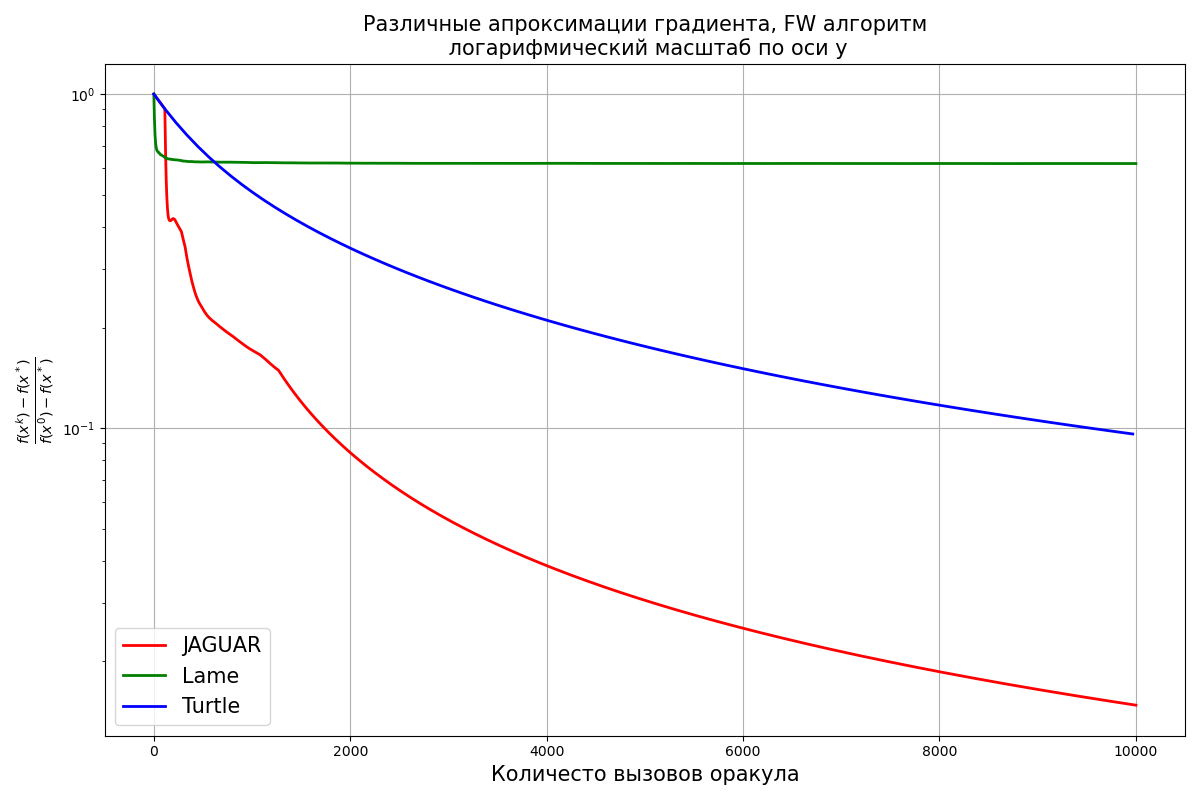
\includegraphics[width = 0.9\textwidth]{BachelorThesis_slides/figures/Non-stochastics.png}
    \end{figure}

\end{frame}

%----------------------------------------------------------------------------------------------------------

\begin{frame}{JAGUAR. Стохастический случай}

    Разностные схемы, которые будут использоваться в алгоритме:

    \begin{itemize}
        \item Двухточечная обратная связь:
            \begin{equation*}
                \widetilde{\nabla}_if_\delta(x, \xi) :=  \dfrac{f_\delta(x + \gamma e_i, \xi) - f_\delta(x - \gamma e_i, \xi)}{2 \gamma} e_i,
            \end{equation*}
        \item Одноточечная обратная связь:
            \begin{equation*}
                \widetilde{\nabla}_if_\delta(x, \xi^+, \xi^-) :=  \dfrac{f_\delta(x + \gamma e_i, \xi^+) - f_\delta(x - \gamma e_i, \xi^-)}{2 \gamma} e_i,
            \end{equation*}
    \end{itemize}

    где $e_i$ - $i$-ый базисный вектор, $\gamma$ - параметр сглаживания.

\end{frame}

%----------------------------------------------------------------------------------------------------------

\begin{frame}{JAGUAR. Стохастический случай}

    \begin{algorithm}[H]
    	\caption{JAGUAR. Стохастический случай}
        \begin{algorithmic}[1]
    		\State {\bf Вход:} $x, h, g \in \mathbb{R}^d$, $0 \leq \eta \leq 1$
      
            \State Сэмплируем $i \in \overline{1, d}$ независимо и равномерно
          
            \State Сэмплируем 2 реализации $\xi$: $\xi^+$ и $\xi^-$ независимо (в случае одноточечной обратной связи $\xi^+= \xi^-$)

            \State Считаем $\widetilde{\nabla}_i f_{\delta}(x, \xi^+, \xi^-) = \frac{f_{\delta}(x + \gamma e_i, \xi^+) - f_{\delta}(x - \gamma e_i, \xi^-)}{2 \gamma} e_i$

            \State $h = h - \dotprod{h}{e_i} e_i + \widetilde{\nabla}_i f_{\delta}(x, \xi^+, \xi^-)$

            \State $\rho = h - d \cdot \dotprod{h}{e_i} e_i + d \cdot \widetilde{\nabla}_i f_{\delta}(x, \xi^+, \xi^-)$

            \State $g = (1 - \eta) g + \eta \rho$
    
            \State \textbf{Выход:} $h$ и $g$ 
        \end{algorithmic}
    \end{algorithm}
  
\end{frame}

%----------------------------------------------------------------------------------------------------------

\begin{frame}{JAGUAR. Стохастический случай}

    Допущения:
        \begin{enumerate}
            \item Функция $f(x, \xi)$ $L(\xi)$-гладкая на множестве $Q$, то есть: 
                \begin{equation*}
                    \forall x, y \in Q \hookrightarrow \left\|\nabla f(x, \xi) - \nabla f(y, \xi)\right\| \leq L(\xi) \left\|x-y\right\|.
                \end{equation*}

            \item Ограниченность оракульного шума:
                \begin{equation*}
                    \exists \Delta > 0 : ~\forall x \in Q \hookrightarrow \expect{|\delta(x, \xi)|^2} \leq \Delta^2
                \end{equation*}

            \item Ограниченность второго момента градиента:
                \begin{equation*}
                    \exists \sigma^2_{\nabla} : \expect{\norms{\nabla f(x, \xi) - \nabla f(x)}^2} \leq \sigma^2_{\nabla}
                \end{equation*}

            \item Ограниченность второго момента градиента:
                \begin{equation*}
                    \exists \sigma^2_{f} : \expect{\left|f(x, \xi) - f(x) \right|^2} \leq \sigma^2_{f}
                \end{equation*}
        \end{enumerate}    

\end{frame}

%----------------------------------------------------------------------------------------------------------

\begin{frame}{Франк-Вульф с JAGUAR в стохастическом случае}
    
    \begin{algorithm}[H]
        \caption{ФВ с JAGUAR в стохастическом случае}
        \begin{algorithmic}[1]
                \State {\bf Вход:} $x_0 \in Q$, $h^0 = g^0 = \widetilde\nabla f_{\delta}(x^0, \xi_1^+, ...., \xi_d^-)$, $\{\eta_k\}_{k=0}^N \subset [0; 1]$
                
        	    \For {k = 0, 1, 2, ... , N}
                    \State $h^{k+1}, g^{k+1} = $ JAGUAR $\left( x^k, h^k, g^k, \eta_k \right)$
                    
                    \State $s^k = \underset{x \in Q}{\arg\min}\left\{\left<s, g^{k+1} \right> \right\}$
                    
                    \State $x^{k+1} = x^k + \gamma_k (s^k - x^k)$ \label{line:x^k}
                \EndFor
            \State \textbf{Выход:} $x^{N+1}$ 
        	\end{algorithmic}
        \end{algorithm}
        
\end{frame}

%----------------------------------------------------------------------------------------------------------

\begin{frame}{JAGUAR. Стохастический случай}

    \textbf{Теорема} При шаге оптимизатора и шаге моментума:
            
        $$\gamma_k = \frac{4}{k + 8d^{3/2}}, \quad \eta_k = \frac{4}{(k + 8d^{3/2})^{2/3}}$$
            
        получается следующее:

        \small{
            \begin{equation*}
                \begin{split}
                    \expect{\norms{g^k - \nabla f(x^k)}^2} 
                    &=
                    \mathcal{O} \Bigg( \frac{d^4 \norms{h^0 - \nabla f(x^0)}^2}{(k + 8d^{3/2})^{8/3}} + d L^2 \gamma^2 + \frac{d \Delta^2}{\gamma^2}
                    \\&+
                    \frac{L^2 D^2 + \max\{d^2 \sigma_f^2/ \gamma^2 + d^2 \sigma_{\nabla}^2, d \norms{g^0 - \nabla f(x^0)}^2\}}{(k + 8d^{3/2})^{2/3}}  
                    \Bigg)
                \end{split} 
            \end{equation*}
        }

        Если $h^0 = g^0 = \widetilde{\nabla} f_\delta(x^0, \xi^+_1, \xi^-_1, ..., \xi^+_d, \xi^-_d)$, то можно упростить:
    
        \begin{equation*}
            \expect{\norms{g^k - \nabla f(x^k)}^2} = \mathcal{O} \left(\frac{L^2 D^2 + d^2 \sigma_f^2/ \gamma^2 + d^2 \sigma_{\nabla}^2}{(k + 8d^{3/2})^{2/3}} + d L^2 \gamma^2 + \frac{d \Delta^2}{\gamma^2} \right)
        \end{equation*}
            
\end{frame}

%----------------------------------------------------------------------------------------------------------

\begin{frame}{Франк-Вульф с JAGUAR в стохастическом случае}

    \textbf{Теорема} При шаге оптимизатора и шаге моментума:
        $$\gamma_k = \frac{4}{k + 8d^{3/2}}, \quad \eta_k = \frac{4}{(k + 8d^{3/2})^{2/3}}$$
            
        получается следующее:
        \small{
            \begin{equation*}
                \begin{split}
                    \expect{f(x^{N}) - f(x^*)} = \mathcal{O}
                    &\Bigg(
                    \frac{L D^2 + d \sigma_f D/ \gamma + d \sigma_{\nabla} D + \sqrt{d} (f(x^0) - f(x^*))}{(N + 8d^{3/2})^{1/3}} 
                    \\&+
                    \sqrt{d} L D \gamma + \frac{\sqrt{d} \Delta D}{\gamma} \Bigg)
                \end{split}
            \end{equation*}
        }

            \textbf{Следствие} Пусть $\varepsilon$ определяет точность, то есть $\expect{f(x^N) - f(x^*)} \leq \varepsilon$. Тогда:

        \small{
            \begin{equation*}
                N = \mathcal{O} \left( \max\left\{ \left[ \frac{L D^2 + d\sigma_{\nabla} D + \sqrt{d} (f(x^0) - f(x^*))}{\varepsilon}\right]^3 , \frac{d^{9/2} \sigma_f^3 L^3D^6}{\varepsilon^6} \right\}\right),
            \end{equation*}
        }
        \small{
            \begin{equation*}
                \gamma = \mathcal{O} \left(\frac{\varepsilon}{\sqrt{d} L D} \right), \quad
                \Delta = \mathcal{O} \left( \frac{\varepsilon^2}{d L D^2}\right).
            \end{equation*}
        }
            
\end{frame}

%----------------------------------------------------------------------------------------------------------

\begin{frame}{Вывод}

    Для задачи выпуклой задачи оптимизации на ограниченном множестве с доступом только к нулевому оракулу предложена и исследована модификация JAGUAR для Франка-Вульфа. Получены теоретические оценки сходимости для нестохастического и стохастического случаев.
    
\end{frame}

%----------------------------------------------------------------------------------------------------------

\begin{frame}{Дальнейшая работа}

    \begin{itemize}
        \item Провести эксперименты на различных множествах, датасетах, функциях;
        \item Возможно, рассмотреть другие методы, например, градиентный спуск.
    \end{itemize}

\end{frame}

%----------------------------------------------------------------------------------------------------------

\end{document}